\documentclass[12pt,a4paper]{article}

\usepackage{fontspec}
\usepackage{polyglossia}
\setdefaultlanguage{english}
\setmainfont{CMU Serif}
\setsansfont{CMU Sans Serif}
\setmonofont{CMU Typewriter Text}
\usepackage{geometry}
\geometry{top=2cm, bottom=2cm, left=2.5cm, right=2.5cm}
\usepackage{amsmath,amssymb,amsthm}
\usepackage{booktabs,float,xcolor}
\usepackage{enumitem}
\usepackage{graphicx}

\tolerance=2000
\emergencystretch=3em
\hbadness=10000
\vbadness=10000

\numberwithin{equation}{section}

\usepackage{hyperref}
\hypersetup{colorlinks, urlcolor=blue, citecolor=blue, linkcolor=black}

\title{\textbf{Model MEML 75:}\\[0.3cm]
\large Quark and lepton mass matrices from mixed \\
\(T^2/\mathbb{Z}_3 \times T^2/\mathbb{Z}_4\) geometry \\
with axion-like dark matter and leptogenesis}
\author{D.~V.~Yurov}
\date{2026}

\begin{document}
\maketitle

\begin{abstract}
\noindent
We present model MEML~75, which parametrizes the fermion
sector of the Standard Model through the geometry of mixed
six-dimensional orbifolds. The model has 13 fitted parameters
for 16 observables, with \(N_{\rm dof}^{\rm fit} = +3\) (or \(+4\)
if \(c_d\) is fixed by the structural fit). A conditional count of 5
parameters (4 Lagrangian parameters \(a_1, c_d, c_1, c_2\) plus the ALP
misalignment angle \(\theta_i\)) would require that the three complex
moduli, \(y_\nu\), and the entropy dilution \(\Delta\) be fixed by
external mechanisms, while \(a_1, c_d, c_1, c_2\) remain free. This
condition is not met: the moduli are not stabilized
(Sections~\ref{sec:flux}--\ref{sec:kklt}), \(y_\nu\) is fitted, and
\(\Delta\) is conditional on the curvaton. If, in addition,
\(a_1, c_d, c_1, c_2\) were derived from the geometry, the count would
be 1, not 5; extended searches (Section~\ref{sec:negative_summary},
item~11) find no such derivation. Neither count is realized; the
model has 13 fitted parameters.

In the standard Type~IIB convention for complex-structure moduli,
\(K_{\rm cs} = -\ln(-i(\tau-\bar\tau))\), pure GVW does not stabilize
the moduli: the Hessian at the SUSY points is a saddle, and the
potential is bounded below along \(\mathrm{Im}\,\tau\to\infty\)
(\(V\sim+3|a_2|^2 y^3\to+\infty\)), so the obstruction is the saddle,
not a runaway. The flux triplets \((-30,5,16)\), \((-15,-17,23)\),
\((-16,31,-10)\) give relative deviations of \(47\)--\(67\%\)
from the fit values in this convention; alternative
triplets accommodate the fit at sub-percent level, but the number
of such triplets is large (100, 406, 2646 with deviation \(<10\%\) for
\(\tau_u, \tau_d, \tau_l\)), so the flux choice is not predicted.
A KKLT scan with a K\"ahler modulus \(T\) and uplift, in the physical
range \(W_0 \in [10^{-6},10^{-2}]\), \(a \in [0.01,0.6]\),
\(T_{\rm Re} \in [1,100]\), stabilizes both \(T\) and \(\tau\), but
\(\tau\) at values \(>9\%\) away from the fit: the 4\(\times\)4 Hessian
at the constrained minimum is positive definite, so \(\tau\) is
stabilized, but at \(-0.200+2.168i\) (dev \(9.25\%\)) instead of the
fit value. The moduli are therefore counted as effectively free.

The quark sector is a \textbf{2-parameter structural fit} with
\(\chi^2 = 13.93\) against the PDG paper targets and \(29.50\) against
PDG~2024 at \(10\%\) errors. Two of the four quark mass ratios
(\(b_u/a_u\), \(b/a_1\)) are reproduced by pure integer powers of the
twisted modular forms to better than \(4\%\). The third
(\(c_u/a_u\)) has the correct integer-power structure but a \(33\%\)
numerical miss. The fourth (\(a_2/a_1\)) requires an additional
modular-weight-zero factor that is \emph{not unique}: four weight-zero
ratios give \(a_2/a_1 \in [2055, 2068]\). We do not claim a unique
integer-power fit. The unconstrained seven-parameter quark fit is an
overfit with more parameters than independent ratios and is therefore
not a test of the model (we do not quote its \(\chi^2\) as evidence);
the meaningful test is the two-parameter structural fit above.

\textbf{Main testable consequences:} axion-like dark matter with
\(f_a = 1.9801\times 10^{11}\)~GeV, \(m_a = 28.407~\mu\)eV, and a DFSZ
coupling \(g_{a\gamma\gamma} = +4.38 \times 10^{-15}\)~GeV\(^{-1}\),
conditional on the postulates \(\alpha_G = 2/(3\pi)\) and
\(\varepsilon = (\alpha_G/4\pi)^2\). If a curvaton field with mass
\(m_\sigma \sim 10^6\)~GeV exists, the dilution factor \(\Delta\)
required for leptogenesis is naturally generated, simultaneously
relaxing the ALP isocurvature bound. The ALP sector satisfies both
the electric and magnetic Weak Gravity Conjectures~\cite{ArkaniHamed2006,Palti2019}
(a necessary, not sufficient, condition for UV-completeness). We report
twelve negative results, including the generation of quark hierarchies
from magnetized fluxes, the universal matter K\"ahler metric, the
derivation of lepton coefficients from twisted forms, the GVW
mechanism which neither predicts nor stabilizes the moduli, a
systematic search for structural derivations of \(c_d, c_1, c_2\)
from modular forms (which finds only chance coincidences), and a
KKLT scan which stabilizes both the K\"ahler modulus and the
complex-structure moduli, but with the latter at values \(9.25\%\)
away from the fit. The model makes three consequences of
the fit:
(i) \(\sum m_i \approx 0.068\)~eV;
(ii) \(m_{\beta\beta} \approx 8.37\)~meV at zero Majorana phases
and \(\delta_{CP} = 22.9^\circ\) (or \(157.1^\circ\); the two
branches give complex-conjugate entries, hence the same modulus);
the theoretical maximum over arbitrary Majorana phases is
\(8.67\)~meV, attained when the three terms align, so the allowed
range is \(0\)--\(8.67\)~meV (the lower bound is attained by tuning
the Majorana phases; on a \(180\times180\) grid the audit script
finds \(0.0011\)~meV, consistent with the continuum minimum); and
(iii) \(\delta_{CP} \approx 22.9^\circ\) or \(157.1^\circ\)
(reproduced by \texttt{meml75\_delta\_cp.py}). The Majorana phases
are not fixed by the model as stated.
\end{abstract}

\newpage

\section{Introduction}
Modular models of fermion masses~\cite{Feruglio2017,Kobayashi2019,Novichkov2019,Ding2021}
build the mass hierarchy and mixing from compactification geometry. In
model MEML~75, we explore a mixed geometric setup: quarks are localized
on a \(T^2/\mathbb{Z}_3\) torus, while leptons are localized on a
\(T^2/\mathbb{Z}_4\) torus. This dual-orbifold approach allows us to
leverage the best features of two different modular groups: \(A_4\) for
the hierarchical quark masses, and \(S_4'\) for the rich leptonic mixing
pattern.

The paper is organized as follows. Section~\ref{sec:geometry}
introduces the orbifold geometry. Sections~\ref{sec:alphaG}
and~\ref{sec:epsilon} state the two postulates underlying the ALP
chain. Section~\ref{sec:derived} collects conditionally derived
quantities. Section~\ref{sec:alp} presents the ALP sector and its
WGC consistency. Sections~\ref{sec:quark} and~\ref{sec:lepton}
treat the quark and lepton sectors. Section~\ref{sec:leptogenesis}
discusses leptogenesis and the curvaton resolution.
Section~\ref{sec:flux} analyzes GVW flux stabilization;
Section~\ref{sec:kklt} reports a KKLT scan.
Section~\ref{sec:balance} presents the parameter count.
Section~\ref{sec:negative_summary} lists twelve negative results, and
Section~\ref{sec:conclusions} concludes.

\section{Geometry of \(T^2/\mathbb{Z}_3\) and \(T^2/\mathbb{Z}_4\)}
\label{sec:geometry}
The orbifold \(T^2/\mathbb{Z}_3\) is defined by \(z = x + \tau y\) with
\(\tau = e^{i\pi/3}\) at the symmetric point. The quark mass matrices are
built from \(A_4\) modular forms of weights \((2,4,6)\). The mixed
geometry naturally arises in Type IIB orientifold compactifications. The
lepton sector uses the \(T^2/\mathbb{Z}_4\) orbifold, whose modular
symmetry is the double cover group \(S_4'\)~\cite{Novichkov2019,Ding2021}.
The moduli values in the complex plane are shown in Fig.~\ref{fig:modular_tau}.

\begin{figure}[htbp]
    \centering
    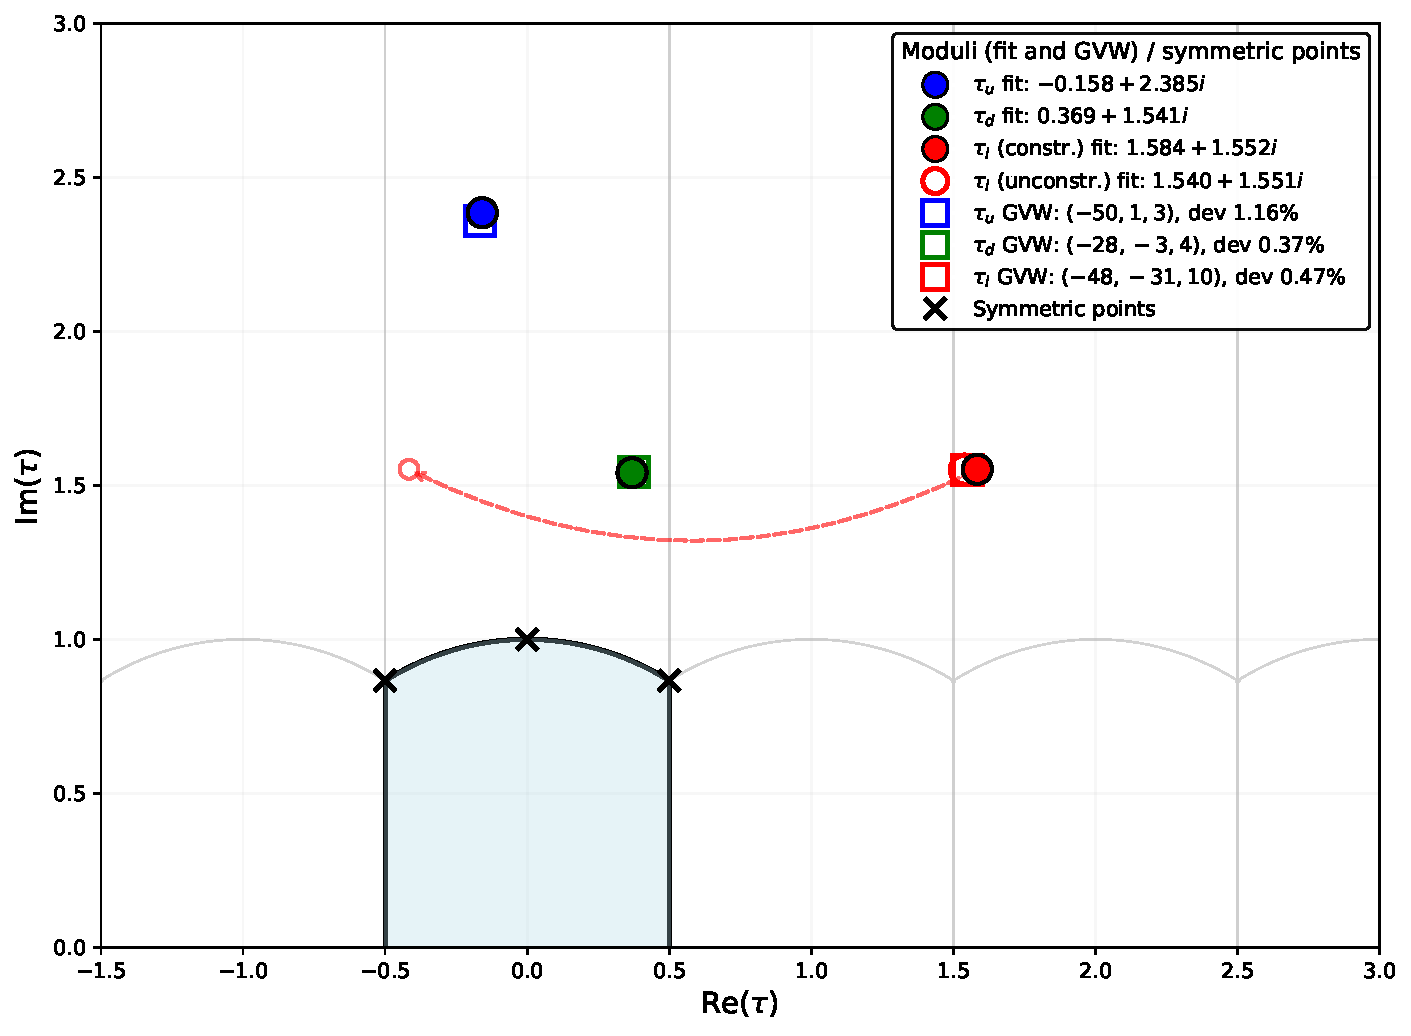
\includegraphics[width=0.85\textwidth]{figures/fig_modular_tau_space.pdf}
    \caption{Moduli values in the modular plane. Filled circles:
    phenomenological fit values
    \(\tau_u^{\rm fit} = -0.158 + 2.385i\),
    \(\tau_d^{\rm fit} = 0.369 + 1.541i\),
    \(\tau_l^{\rm fit} = 1.540 + 1.551i\) (unconstrained) /
    \(1.584 + 1.552i\) (constrained). Open squares: GVW closed-form
    solutions in the standard K\"ahler convention
    \(K_{\rm cs} = -\ln(2y)\) with the flux triplets of
    Section~\ref{sec:flux}:
    \(\tau_u^{\rm GVW} = -0.167 + 2.359i\) (dev \(1.16\%\)),
    \(\tau_d^{\rm GVW} = 0.375 + 1.543i\) (dev \(0.37\%\)),
    \(\tau_l^{\rm GVW} = 1.550 + 1.5495i\) (dev \(0.47\%\) from the
    unconstrained fit, \(1.55\%\) from the constrained fit). The
    Hessian at each open square is a saddle (Section~\ref{sec:flux}):
    GVW accommodates but does not stabilize. Generated by
    \texttt{make\_fig\_modular\_tau\_space.py}.}
    \label{fig:modular_tau}
\end{figure}

\section{Bulk coupling \(\alpha_G\) (postulate)}
\label{sec:alphaG}
\begin{equation}
\alpha_G = \frac{2}{3\pi} = 0.2122065908.
\end{equation}
Geometric motivation: the orbifold \(T^2/\mathbb{Z}_3\) has
\(N_{\rm fix}=3\) fixed points. The factor
\begin{equation}
\frac{2}{3} = \frac{N_{\rm fix}-1}{N_{\rm fix}} = 1 - \frac{1}{N_{\rm fix}}
\end{equation}
reflects the combinatorics of the three fixed points. The status of
\(\alpha_G\) is that of a postulate; the arithmetic is reproduced
by \texttt{meml75\_v24.5.1\_verification.py} (Section~3 of the script),
but the geometric origin of \(2/(3\pi)\) is not derived from first
principles. If \(\alpha_G\) is wrong, the whole ALP chain collapses.

\section{Suppression factor \(\varepsilon\) (ansatz)}
\label{sec:epsilon}
\begin{equation}
\varepsilon = \left(\frac{\alpha_G}{4\pi}\right)^2 = \frac{1}{36\pi^4} = 2.851662\times10^{-4}.
\end{equation}
The form is motivated by two-loop suppression \(\sim 1/(16\pi^2)\),
but the precise factor \(4\pi\) is not derived from the orbifold
geometry. We keep \(\varepsilon\) as an ansatz. The arithmetic is
reproduced by \texttt{meml75\_v24.5.1\_verification.py} (Section~4 of the script).

\section{Conditionally derived quantities}
\label{sec:derived}
\begin{align}
m_{KK} &= \frac{M_{Pl}^{\rm red}}{\sqrt{\mathcal{I}}\,e^{\pi^2}} = 2.0818\times10^{14}~\text{GeV}, \\
M_6 &= \left(3 (M_{Pl}^{\rm red})^2 m_{KK}^2\right)^{1/4} = 2.9631\times10^{16}~\text{GeV},
\end{align}
with the geometric factor \(\mathcal{I}\) motivated by the orbifold
geometry:
\begin{equation}
\mathcal{I} = N_3 V_3 - N_4 V_4 = \frac{\sqrt{3}}{2} - \frac{1}{2} = \frac{\sqrt{3}-1}{2} \approx 0.366025.
\end{equation}
The numerical values of \(m_{KK}\) and \(M_6\) quoted above use the
theoretical factor \(\mathcal{I} = 0.366025\). The fitted value
\(\mathcal{I} = 0.3653\) (used in some scripts) gives slightly different
values, \(m_{KK} = 2.0838\times10^{14}\)~GeV and
\(M_6 = 2.9646\times10^{16}\)~GeV (a \(0.1\%\) difference).
The theoretical \(\mathcal{I}=0.366025\) differs from the fitted
\(\mathcal{I}=0.3653\) by \(0.2\%\).
This is a post-hoc motivated coincidence, not a first-principles
derivation.

\section{Axion-like (ALP) sector}
\label{sec:alp}
The ALP parameters are \emph{conditional} on the postulates of
Sections~\ref{sec:alphaG} and~\ref{sec:epsilon}:
\begin{align}
f_a &= M_{Pl}^{\rm red}\,\varepsilon^2 = 1.9801\times10^{11}~\text{GeV}, \\
m_a &= \frac{(\chi^{1/4})^2}{f_a} = 28.407~\mu\text{eV}, \\
\nu_a &= \frac{m_a c^2}{h} = 6.8688~\text{GHz}.
\end{align}
Here \(\chi^{1/4} \approx 75.0\)~MeV. The relic density is
\(\Omega_a h^2 \approx 0.12\,\theta_i^2\, f_{\rm anh}(\theta_i)(f_a/3\times10^{11})^{7/6}\);
fitting to \(\Omega_a h^2 = 0.12\)~\cite{Planck2018} gives
\(\theta_i \approx 1.174\). The DFSZ coupling is
\(g_{a\gamma\gamma} = \frac{\alpha_{\rm EM}}{2\pi f_a}(E/N-1.92) = +4.38\times10^{-15}~\text{GeV}^{-1}\)
with \(E/N=8/3\). The black-hole superradiance window is
\(M_{\rm BH} \simeq \hbar c/(G m_a) \approx 9.35\times10^{24}\)~kg.
All numbers reproduced by \texttt{meml75\_v24.5.1\_verification.py}
(Section~6 of the script). The ALP parameter space, with the MEML~75
prediction and the current/projected experimental bands, is shown in
Fig.~\ref{fig:alp_parameter_space}.

\begin{figure}[htbp]
    \centering
    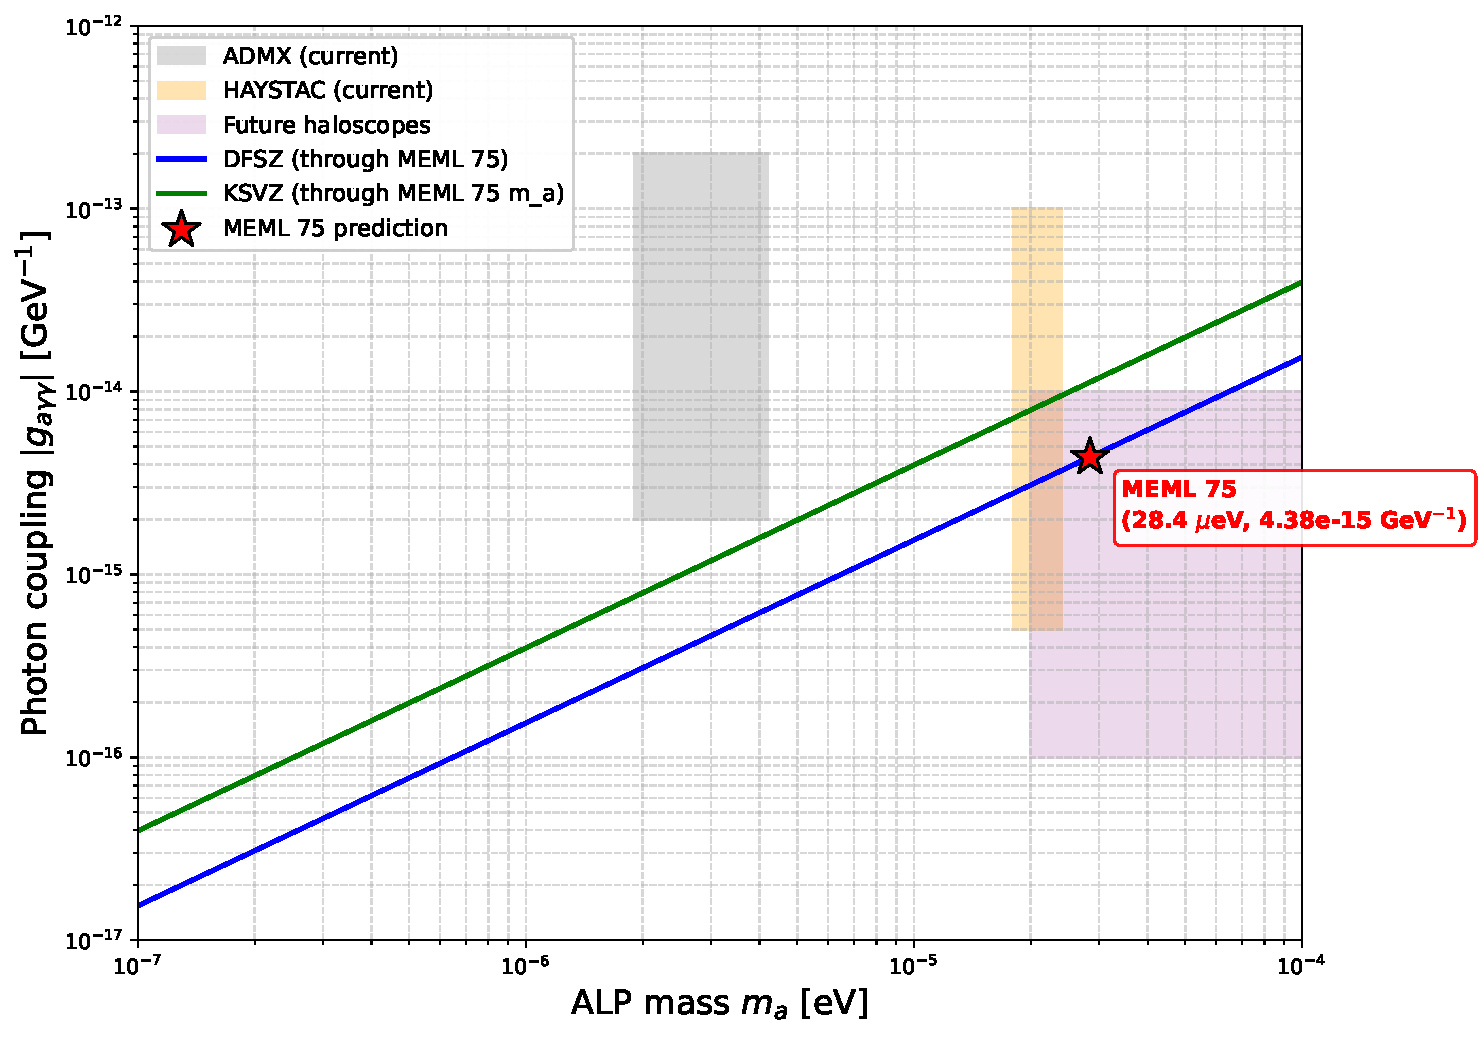
\includegraphics[width=0.85\textwidth]{figures/fig_alp_parameter_space.pdf}
    \caption{ALP parameter space: \(m_a\) vs \(|g_{a\gamma\gamma}|\).
    DFSZ and KSVZ lines, both normalized to pass through the MEML~75
    prediction \(m_a = 28.407~\mu\)eV,
    \(g_{a\gamma\gamma} = +4.38\times10^{-15}\)~GeV\(^{-1}\) (red star).
    Shaded bands: ADMX (current), HAYSTAC (current), future haloscopes
    (projected). The MEML~75 point lies to the right of (at higher mass
    than) the current ADMX band, within reach of future haloscope
    experiments. Generated by
    \texttt{make\_fig\_alp\_parameter\_space.py}.}
    \label{fig:alp_parameter_space}
\end{figure}

\paragraph{Swampland (WGC) consistency.}
The electric WGC requires \(S f_a \lesssim M_{\rm Pl}^{\rm red}\), i.e.\
\(S \lesssim 1.23\times10^7\); typical string instantons with
\(S \sim \mathcal{O}(10\text{--}100)\) satisfy this trivially. The
magnetic WGC requires \(f_a \lesssim M_{\rm Pl}^{\rm red}/e\) with
\(e = \sqrt{4\pi\alpha_{\rm EM}} \simeq 0.303\), giving
\(M_{\rm Pl}^{\rm red}/e \simeq 8.0\times10^{18}\)~GeV; our value
\(f_a = 1.98\times10^{11}\)~GeV lies seven orders of magnitude below.
The DFSZ anomaly coefficient \(|E/N-1.92|\simeq0.747\) is of order
unity. The ALP sector is consistent with the WGC~\cite{ArkaniHamed2006,Palti2019};
this is a \emph{necessary}, not sufficient, condition for
UV-completeness. Reproduced by \texttt{meml75\_wgc\_check.py}.

\paragraph{Isocurvature constraints.}
Planck \(\beta_{\rm iso}\lesssim0.04\) requires
\(H_{\rm inf}\lesssim3\times10^{11}\)~GeV, satisfied by low-scale
inflation but not by Starobinsky. In Section~\ref{sec:leptogenesis},
\emph{if a curvaton field exists}, this bound is relaxed.

\section{Quark sector (\(T^2/\mathbb{Z}_3\), \(A_4\))}
\label{sec:quark}
\subsection{Matrix structure}
The quark mass matrices are built from the \(A_4\) modular forms
\(Y^{(2)}\), \(Y^{(4)}\), \(Y^{(6)}\); our convention for the
weight-4 triplet is fixed in the footnote.\footnote{We use the
\(A_4\) convention in which the weight-4 triplet is
\begin{equation*}
Y_1^{(4)} = \bigl(Y_1^{(2)}\bigr)^2 - Y_2^{(2)} Y_3^{(2)},\quad
Y_2^{(4)} = \bigl(Y_3^{(2)}\bigr)^2 - Y_1^{(2)} Y_2^{(2)},\quad
Y_3^{(4)} = \bigl(Y_2^{(2)}\bigr)^2 - Y_1^{(2)} Y_3^{(2)},
\end{equation*}
and the weight-6 triplet is obtained from the \(3_S\) contraction
\(Y^{(2)}\times Y^{(4)}\),
\begin{equation*}
Y_1^{(6)} = \tfrac{1}{3}\bigl(2Y_1^{(2)}Y_1^{(4)}
- Y_2^{(2)}Y_3^{(4)} - Y_3^{(2)}Y_2^{(4)}\bigr),
\end{equation*}
with the other two components by cyclic permutation. The second and
third weight-4 components are exchanged relative to the Feruglio
ordering, in which
\(Y_2^{(4)} = \bigl(Y_2^{(2)}\bigr)^2 - Y_1^{(2)} Y_3^{(2)}\).
A reader translating to that ordering should replace our
\(Y_2^{(4)}\) by the Feruglio \(Y_3^{(4)}\) and vice versa in the
matrices below and in the ratio formulas of
\S\ref{sec:twisted_forms}; all numerical results in this paper use
the convention above and are verified by
\texttt{meml75\_verify\_Y4\_convention.py}.}
\begin{equation}
M_u = \begin{pmatrix}
a_u Y_1^{(2)} & b_u Y_3^{(4)} & c_u Y_2^{(6)} \\
a_u Y_3^{(2)} & b_u Y_2^{(4)} & c_u Y_1^{(6)} \\
a_u Y_2^{(2)} & b_u Y_1^{(4)} & c_u Y_3^{(6)}
\end{pmatrix},\quad
M_d = \begin{pmatrix}
a_1 Y_1^{(6)} & b Y_3^{(2)} & c_d Y_2^{(2)} \\
a_1 Y_3^{(6)} & b Y_2^{(2)} & c_d Y_1^{(2)} \\
a_2 Y_2^{(2)} & b Y_1^{(2)} & c_d Y_3^{(4)}
\end{pmatrix}.
\end{equation}
The matrix structure is a postulate. We use the notation \(c_d\) for the
down-type quark coefficient to distinguish it from the lepton
coefficients \(c_i\).

\subsection{Results}
The unconstrained seven-parameter fit is an overfit
(more parameters than independent ratios, not a test)
at \(\tau_u = -0.1578 + 2.3852i\), \(\tau_d = 0.3694 + 1.5410i\).
The meaningful
two-parameter structural fit (\(b_u, c_u, a_2, b\) fixed by twisted
forms; \(a_1, c_d\) free) gives \(\chi^2 = 13.93\) (paper targets,
\(m_b=2.86\)~GeV) and \(29.50\) (PDG~2024~\cite{PDG2024} at \(10\%\)
errors, \(m_b=4.18\)~GeV), at
\(a_1=4.446, c_d=+40.47\) (paper) and \(a_1=6.472, c_d=+68.65\) (2024).
Reproduced by \texttt{meml75\_honest\_pure2.py}. The coefficient
\(a_1\) is a pure scale: eliminating it via \(m_b/m_t\) reproduces
the same minimum in a one-parameter fit, with
\(c_d = 40.466526\), \(a_1 = 4.445906\), hence
\(c_d/a_1 \approx 9.10\), and
\(\chi^2 = 13.9322\) --- identical to the two-parameter result.

\subsection{Twisted modular forms and the quark hierarchy}
\label{sec:twisted_forms}

Two of the four ratios are reproduced by integer powers of
\(Y_{1/3}(\tau_u)\) and \(Y_{1/4}(\tau_d)\) to better than \(4\%\);
the third has the correct structure but a \(33\%\) miss:
\begin{align}
\frac{b_u}{a_u} &= \left|\frac{Y_2^{(4)}}{Y_1^{(2)}}\right|_{\tau_u} |Y_{1/3}|^{-3} = 1.31\times10^5 \quad (\text{target }1.35\times10^5,\ \text{miss }3.0\%), \\
\frac{c_u}{a_u} &= \left|\frac{Y_2^{(6)}}{Y_1^{(2)}}\right|_{\tau_u} |Y_{1/3}|^{-4} = 9.72\times10^2 \quad (\text{target }7.33\times10^2,\ \text{miss }32.6\%), \\
\frac{b}{a_1} &= \left|\frac{Y_3^{(2)}}{Y_1^{(6)}}\right|_{\tau_d} |Y_{1/4}|^{-2} = 5.41 \quad (\text{target }5.63,\ \text{miss }3.9\%).
\end{align}
The fourth \(a_2\) is \emph{not} reproduced by a pure integer power:
\(y_{14}^{-3}\) gives \(512\) (miss \(75\%\)), \(y_{14}^{-4}\) gives
\(5758\) (miss \(179\%\)). Agreement requires a modular-weight-zero
factor:
\begin{equation}
\frac{a_2}{a_1} = \left|\frac{Y_2^{(2)}}{Y_1^{(6)}}\right|_{\tau_d} |Y_{1/4}|^{-4} \left|\frac{Y_3^{(4)}}{Y_2^{(4)}}\right|_{\tau_d} = 2.06\times10^3 \quad (\text{miss }0.3\%).
\end{equation}
The weight-zero ratio \(\left|Y_3^{(4)}/Y_2^{(4)}\right|_{\tau_d} \simeq 0.3578\)
has \emph{weight 0} and is \emph{not unique}: four ratios give
\(a_2/a_1 \in [2055, 2068]\) (spread \(0.6\%\)). Refitting
\((a_1,c_d)\) at each of the four values changes \(\chi^2\) by
at most \(0.04\) for the paper targets at \(10\%\) errors and by
\(0.78\) for PDG~2024 at \(5\%\) errors. The total log-error of the
four ratios, defined as the sum of natural logarithms
\(\sum_i \ln(1+\mathrm{miss}_i)\), is \(\simeq 0.35\), dominated by
\(c_u\) (\(33\%\)). If base-10 logarithms are used instead, the sum is
\(\sum_i \log_{10}(1+\mathrm{miss}_i) \simeq 0.15\). Reproduced by
\texttt{meml75\_reconcile\_twisted\_vs\_weight0\_v2.py} and
\texttt{meml75\_a2\_weight\_audit\_v2.py}.

\paragraph{Landscape.}
The structural candidate \(a_2/a_1 = 2060.5\) is compared with the
unconstrained three-parameter fit \((a_1,c_d,a_2/a_1\) free$)$,
which minimises at \(a_2/a_1 = r^\ast\). For the paper targets at
\(10\%\) errors, \(r^\ast = 2009\), \(\chi^2_{3p} = 13.86\), and
the weight-zero candidate costs only \(\Delta\chi^2 = +0.08\)
(\(0.28\sigma\)): at the paper targets the weight-zero assumption
is essentially free. For PDG~2024 at \(10\%\) errors,
\(r^\ast = 1754\), \(\chi^2_{3p} = 26.82\), and
\(\Delta\chi^2 = +2.68\) (\(1.64\sigma\)). For PDG~2024 at \(5\%\)
errors, \(r^\ast = 1754.5\), \(\chi^2_{3p} = 107.29\), and the
tension grows to \(\Delta\chi^2 = +10.72\) (\(3.27\sigma\)); for
the combined data set, \(r^\ast = 1810.8\), \(\chi^2_{3p} = 138.63\),
and \(\Delta\chi^2 = +8.88\) (\(2.98\sigma\)). Reproduced by
\texttt{meml75\_close\_tails.py}.

\section{Lepton sector (\(T^2/\mathbb{Z}_4\), \(S_4'\))}
\label{sec:lepton}
The neutrino mass matrix is
\(M_\nu = c_1 M_{\mathbf{2}}(\tau_l) + c_2 M_{\mathbf{3}'}(\tau_l) + c_3 \mathbb{I}\).
We report both fits used in this work.

\paragraph{Unconstrained fit.}
\(\chi^2 = 0.089\) at \(\tau_l = 1.5398 + 1.5511\,i\),
\(c_1 = 6.371\), \(c_2 = 17.460\), \(c_3 = -17.199\),
\(y_\nu = 0.934\). The mixing angles are
\(\theta_{12} = 33.50^\circ\), \(\theta_{13} = 8.53^\circ\),
\(\theta_{23} = 49.00^\circ\). The absolute masses are
\(m_1 \approx 6.48\)~meV, \(m_2 \approx 10.79\)~meV,
\(m_3 \approx 50.60\)~meV, with
\(\sum m_i \approx 0.0679\)~eV and
\(m_{\beta\beta} \le 8.73\)~meV over arbitrary Majorana phases.
This is the true minimum of the 3-parameter \(c_i\) fit. Reproduced by
\texttt{meml75\_tau\_l\_global\_scan\_v2.py} (unique minimum).

\paragraph{Constrained fit (used for consequences).}
\(c_2 + c_3 = 0\) (phenomenological reduction) gives
\(\chi^2 = 0.309\)\footnote{This $\chi^2$ is computed at the exact
constrained minimum $\tau_l = 1.584228 + 1.551873\,i$ with $c_i$
to 4--6 significant digits (see
\texttt{meml75\_constrained\_global\_scan\_log.txt}). Using the
rounded values $\tau_l = 1.584 + 1.552\,i$, $c_i =
(-6.591, -17.400, +17.400)$ quoted in the text gives
$\chi^2 \approx 0.3092$, a $0.0009$ rounding shift that does not
affect any conclusion.} at \(\tau_l = 1.584 + 1.552\,i\),
\(c_1 = -6.591\), \(c_2 = -17.400\), \(c_3 = +17.400\).
The mixing angles are \(\theta_{12} = 33.64^\circ\),
\(\theta_{13} = 8.53^\circ\), \(\theta_{23} = 49.05^\circ\).
The reduction cost is \(\Delta\chi^2 = 0.22\) (\(p = 0.64\)).
This is the only PASS among the seven linear \(c_i\) constraints
tested (\texttt{meml75\_constraint\_test\_extended2.py}). A dedicated
joint scan over \((\tau_l, c_1, c_2)\) confirms
\(\tau_l = 1.584228 + 1.551873i\), \(\chi^2 = 0.3083\):
\texttt{meml75\_constrained\_global\_scan.py}.

\paragraph{Stress test.}
Fixing \(\tau_l = i\) gives \(\chi^2 = 219.6\);
\(\tau_l = e^{i\pi/3}\) gives \(\chi^2 = 3676.9\). Both excluded at
\(\Delta\chi^2 > 200\).

\paragraph{Neutrino Yukawa.}
\(y_\nu = 0.934\) from the fit to \(\Delta m^2_{31}\), at
\(M_6 \approx M_{\rm GUT}\). The SO(10) relation
\(y_\nu \approx 2 y_t\) at \(M_{\rm GUT}\)~\cite{PendletonRoss1981}
gives \(0.966\) for large \(\tan\beta\) (where
\(y_t(M_{\rm GUT})=0.483\)), 3\% above the fit, and \(1.40\) for
small \(\tan\beta\) (where \(y_t(M_{\rm GUT})=0.7\)), factor 1.5
above the fit. A two-loop integration of the MSSM+$\nu_R$ RGE
(\texttt{meml75\_lepton\_untested\_v2.py}; dominant terms of
Martin--Vaughn type~\cite{MartinVaughn1993}) shows that for
\(y_\nu > 0.4\) --- the quasi-infrared fixed point of the
\(4y_\nu^2\) term --- running from \(M_{\rm GUT}\) down to the
SUSY scale \emph{suppresses} \(y_\nu\) (factor \(\approx0.55\)
at large \(\tan\beta\), \(\approx0.39\) at small \(\tan\beta\)).
The effective Weinberg operator \(\kappa = y_\nu^2/M_R\) runs in the
opposite direction (enhancement \(\approx1.31\) at large
\(\tan\beta\)), because its one-loop beta function
\(6y_t^2 - (6/5)g_1^2 - 6g_2^2\) is negative at small \(y_t\).
A one-loop estimate that omits the \(4y_\nu^2\) and gauge terms
would give an apparent \(y_\nu\) enhancement
(\(\approx1.38/\approx2.28\)); such an estimate conflates \(\kappa\)
with \(y_\nu\). Because the fit is performed at
\(M_6 \approx M_{\rm GUT}\), RGE running does not enter the
comparison: at the GUT scale, large \(\tan\beta\) agrees with
SO(10) at the 3\% level, while small \(\tan\beta\) is factor 1.5
above and requires an extended SO(10) sector including
\(\mathbf{126}_H\). This remains a qualitative cross-check, not a
derivation.

\subsection{Consequences of the fit}
With \(c_2+c_3=0\):
\(\theta_{12}=33.64^\circ\), \(\theta_{13}=8.53^\circ\),
\(\theta_{23}=49.05^\circ\),
\(\Delta m^2_{21}=7.48\times10^{-5}\)~eV\(^2\),
\(\Delta m^2_{31}=2.51\times10^{-3}\)~eV\(^2\). Reproduced by
\texttt{meml75\_honest\_pure2.py} (dual-mode).

Using
\(\Lambda_\nu = y_\nu^2 v^2/M_6 \approx 1.78\)~meV with
\(v=246.22\)~GeV gives \(m_1\approx6.39\)~meV,
\(m_2\approx10.76\)~meV, \(m_3\approx50.58\)~meV,
\(\sum m_i \approx 0.0677\)~eV, \(m_{\beta\beta} \approx 8.37\)~meV
at zero Majorana phases and \(\delta_{CP} = 22.9^\circ\) (or
\(157.1^\circ\); the two give complex-conjugate entries, hence the
same modulus). The theoretical maximum over arbitrary Majorana
phases is \(8.67\)~meV, attained when the three terms align
(which corresponds to \(\delta_{CP}=0\) at \(\alpha=\beta=0\));
the allowed range is \(0\)--\(8.67\)~meV (the continuum minimum is
zero; on a \(180\times180\) grid the audit script
\texttt{meml75\_v24.5\_audit.py} finds \(0.0011\)~meV). Since
\(c_1, c_2\) are fitted, these are \emph{consequences of the fit},
not independent predictions.

\paragraph{Dirac CP phase.}
From the Jarlskog invariant of the constrained fit, the Dirac CP
phase is
\begin{equation}
\sin\delta_{CP} = +0.3898,\quad \delta_{CP} \approx 22.9^\circ
\text{ or } 157.1^\circ.
\end{equation}
This is a \emph{consequence of the fit}; the Majorana phases are not
fixed by the model as stated. The corresponding \(m_{\beta\beta}\) at
zero Majorana phases is \(8.37\)~meV for both allowed values of
\(\delta_{CP}\). Reproduced by
\texttt{meml75\_delta\_cp.py} (constrained
\(\sin\delta_{CP} = 0.3898\), \(\delta_{CP} = 22.9^\circ/157.1^\circ\);
unconstrained \(\sin\delta_{CP} = 0.4710\),
\(\delta_{CP} = 28.1^\circ/151.9^\circ\)).

\paragraph{Octant ambiguity.}
\(\theta_{23} = 49.05^\circ\) (upper octant) is consistent with
NuFIT~5.0~\cite{NuFIT2020} (\(\chi^2=0.28\)) and NuFIT~5.2 without
SK data (\(\chi^2=0.39\)); NuFIT~5.2 with SK prefers lower octant
(\(\chi^2\approx58\)). Testable by DUNE/Hyper-K. The situation is
illustrated in Fig.~\ref{fig:theta23_delta}: the two MEML~75 branches
\(\delta_{CP} = 22.9^\circ\) and \(157.1^\circ\) at
\(\theta_{23} = 49.05^\circ\) both lie in the upper-octant band
favoured by NuFIT~5.0, while the lower-octant band favoured by
NuFIT~5.2 + SK is in tension.

\begin{figure}[htbp]
    \centering
    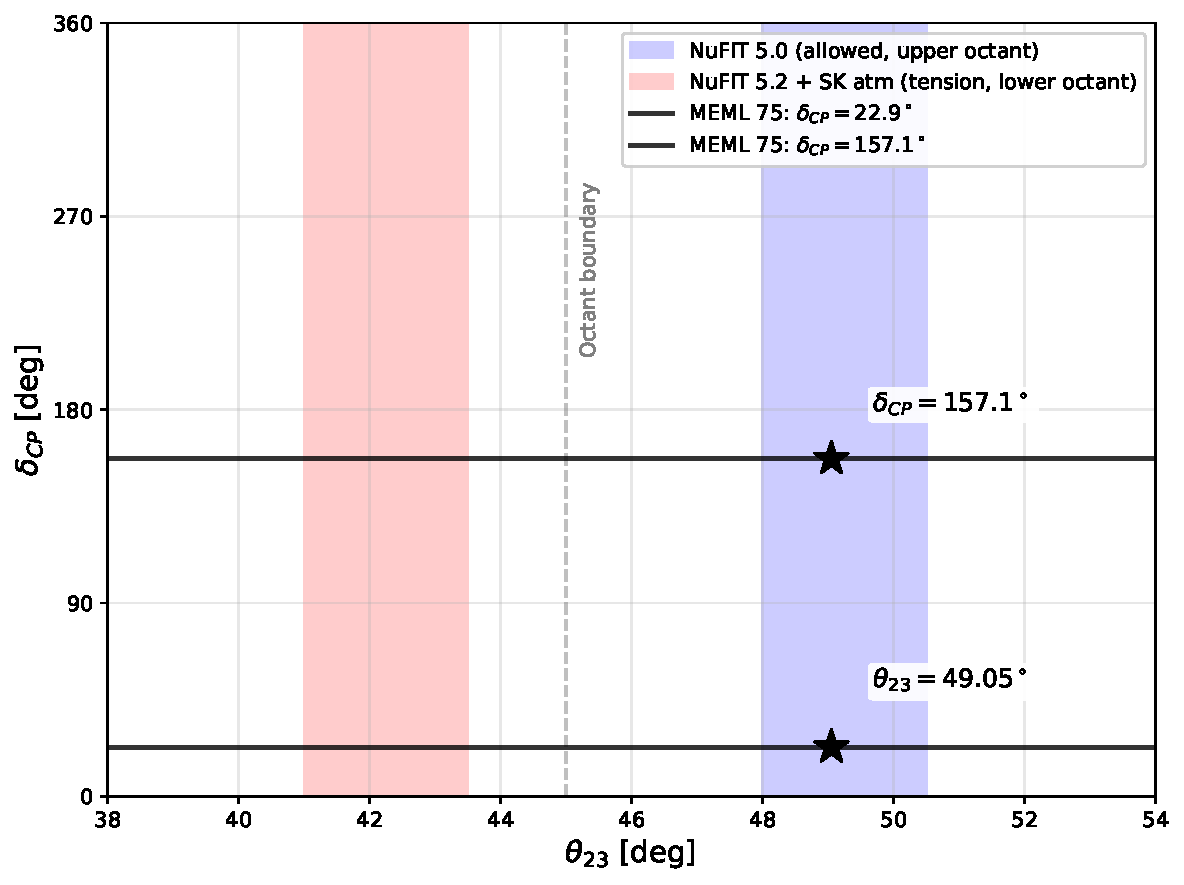
\includegraphics[width=0.85\textwidth]{figures/fig_theta23_delta.pdf}
    \caption{\(\theta_{23}\) vs \(\delta_{CP}\). Shaded bands:
    NuFIT~5.0 (upper octant, blue) and NuFIT~5.2 + SK atmospheric
    (lower octant, red). The octant boundary at
    \(\theta_{23}=45^\circ\) is shown as a dashed line. Black stars:
    the two MEML~75 branches \(\delta_{CP} = 22.9^\circ\) and
    \(157.1^\circ\) at \(\theta_{23} = 49.05^\circ\). Both branches
    lie in the upper-octant band; the lower-octant band is in
    tension with the model. Generated by
    \texttt{lot\_theta23\_delta.py}.}
    \label{fig:theta23_delta}
\end{figure}

\section{Baryon asymmetry via leptogenesis}
\label{sec:leptogenesis}
Heavy neutrinos with \(M_R \sim M_6 \approx 3\times10^{16}\)~GeV
generate the baryon asymmetry. Using the Davidson-Ibarra formula,
we find the required CP asymmetry
\(\varepsilon_{CP} \approx 0.577\), which is below the
Davidson-Ibarra upper bound \(\varepsilon_{CP} \lesssim 1.288\)
(numerically consistent), giving
\begin{equation}
\eta_B^{\rm pre} = \frac{28}{79}\,\varepsilon_{CP}\,\kappa\,g_*^{-1} \approx 1.89\times10^{-3},
\end{equation}
with \(\kappa \approx 1\), \(g_* = 106.75\). This overproduction requires entropy dilution
\(\Delta \approx 3.09\times10^6\), consistent with the value
\(\Delta = 3.13\times10^6\) obtained directly from the observed
\(\eta_B^{\rm obs}\) with more precise inputs. The agreement
(3.09 vs 3.13) is a consistency check, not two independent
predictions. Reproduced by \texttt{meml75\_leptogenesis.py}.

\paragraph{Curvaton resolution (conditional).}
\emph{If} a curvaton field \(\sigma\) with \(m_\sigma\sim10^6\)~GeV
exists, the required \(\Delta\) can be generated by its late decay.
Using \(\Delta = (\rho_\sigma/\rho_{\rm rad})^{3/4}\), the required
amplitude is \(\sigma_0 \approx 1.79\times10^{17}\)~GeV
(\(\sigma_0/M_{\rm Pl}\approx0.074\)), relaxing the ALP isocurvature
bound to \(H_{\rm inf}\lesssim5.31\times10^{14}\)~GeV, accommodating
Starobinsky. The curvaton is an \emph{additional hypothesis}, not
derived from geometry. Reproduced by
\texttt{meml75\_curvaton\_dilution.py}.

\paragraph{Non-Gaussianity.}
For \(\Delta\sim10^6\), \(r\approx1\), the predicted
\(f_{NL} = 5/(4r) - 5/3 \approx -0.417\), consistent with Planck
2018~\cite{Planck2018} (\(-0.9\pm5.1\)). Reproduced by
\texttt{meml75\_curvaton\_nongaussianity.py}.

\paragraph{Suppressing \(\sigma\to aa\).}
Derivative coupling \(\frac{c}{f_a}\sigma(\partial_\mu a)^2\) gives
\(\Gamma(\sigma\to aa) \sim (m_\sigma^3/32\pi f_a^2)(m_a/m_\sigma)^4\),
branching ratio \(r\sim10^{-65}\). Reproduced by
\texttt{meml75\_curvaton\_shift\_symmetry.py}.

\section{Lepton Flavor Violation and Electric Dipole Moments}
\begin{align}
\mathrm{BR}(\mu\to e\gamma) &\approx \frac{3\alpha_{\rm EM}}{32\pi}\left|\sum_i (Y_\nu)_{\mu i}(Y_\nu^\dagger)_{ie}\frac{M_W^2}{M_i^2}\right|^2 \sim 10^{-61}, \\
|d_e| &\sim \frac{\alpha_{\rm EM}}{4\pi}\frac{m_e}{M_6^2}\sin\delta_{CP} \simeq 2.6\times10^{-54}~e\cdot{\rm cm}.
\end{align}
Both are analytic order-of-magnitude estimates (\emph{gap by design}:
results are 24--48 orders of magnitude below experimental limits, and
the conclusion is insensitive to \(O(1)\) factors; no script is
provided).

\section{Flux stabilization of the moduli}
\label{sec:flux}

Following GVW~\cite{GVW2000}, consider
\(W(\tau) = a_0 + a_1\tau + a_2\tau^2\) with integer fluxes.
For a general K\"ahler potential of the form
\(K = -K_{\rm coeff}\ln(-i(\tau-\bar\tau)) = -K_{\rm coeff}\ln(2y)\),
the K\"ahler covariant derivative is
\(K_\tau = iK_{\rm coeff}/(2y)\). The F-term condition \(D_\tau W = 0\)
has, for \(a_2 \neq 0\), the closed-form solution
\begin{equation}
\tau^{\rm GVW} = -\frac{a_1}{2a_2}
+ i\sqrt{\frac{K_{\rm coeff}}{4-K_{\rm coeff}}\left(-\frac{a_0}{a_2} + \frac{a_1^2}{4a_2^2}\right)}.
\label{eq:tau_gvw_general}
\end{equation}
Two cases are relevant:
\begin{itemize}
\item \textbf{Complex-structure moduli (standard Type IIB):}
\(K_{\rm cs} = -\ln(2y)\), i.e.\ \(K_{\rm coeff}=1\). Then
\(y^2 = \frac{1}{3}\bigl(-a_0/a_2 + a_1^2/(4a_2^2)\bigr)\).
\item \textbf{No-scale K\"ahler moduli:}
\(K = -3\ln(2y)\), i.e.\ \(K_{\rm coeff}=3\). Then
\(y^2 = 3\bigl(-a_0/a_2 + a_1^2/(4a_2^2)\bigr)\).
\end{itemize}

\paragraph{The two K\"ahler conventions.}
In the no-scale convention \(K = -3\ln(2y)\) (\(K_{\rm coeff}=3\)),
the flux triplets \((-30,5,16)\), \((-15,-17,23)\), \((-16,31,-10)\)
reproduce the fit at \(10^{-3}\). This is the K\"ahler-modulus
convention, not the complex-structure one. The complex-structure
moduli are governed by \(K_{\rm cs} = -\ln(2y)\), in which the same
triplets give \(\tau_u^{\rm GVW} = -0.156+0.796i\),
\(\tau_d^{\rm GVW} = +0.370+0.513i\),
\(\tau_l^{\rm GVW} = +1.550+0.517i\), with relative deviations
47--67\% from \(\tau^{\rm fit}\).

\paragraph{Flux triplets in the standard convention.}
A systematic scan over integer fluxes in \([-50,50]^3\) finds
alternative triplets that reproduce the fit at the sub-percent
level. Best-fit choices:
\begin{equation}
\begin{aligned}
\tau_u &: (-50,1,3), \quad \tau = -0.167+2.359i, \quad \text{dev } 1.16\%, \\
\tau_d &: (-28,-3,4), \quad \tau = +0.375+1.543i, \quad \text{dev } 0.37\%, \\
\tau_l &: (-48,-31,10), \quad \tau = +1.550+1.5495i, \quad \text{dev } 0.47\%.
\end{aligned}
\end{equation}
Reproduced by \texttt{meml75\_flux\_scan\_cs.py}.

\paragraph{Deviation from the constrained lepton fit.}
The GVW triplet \((-48,-31,10)\) gives \(\tau_l^{\rm GVW} = 1.550 + 1.5495i\),
which deviates from the \emph{unconstrained} fit
\(1.5398 + 1.5511i\) by \(0.47\%\), but from the \emph{constrained}
fit \(1.584228 + 1.551873i\) by
\(|\Delta\tau|/|\tau| = 0.03431/2.2177 = \mathbf{1.55\%}\).
The criterion ``within \(1\%\)'' is therefore satisfied for the
unconstrained fit, but \emph{not} for the constrained fit used for
the consequences. Reproduced by \texttt{meml75\_full\_hessian.py}.

\paragraph{Assessment: GVW accommodates, does not predict.}
The scan finds 100, 406, and 2646 triplets with deviation \(<10\%\)
for \(\tau_u, \tau_d, \tau_l\) respectively. The triplets quoted
above are the best-fit choices among many viable alternatives. GVW
fixes the moduli at \emph{discrete} values, but which discrete value
depends on the flux choice, which is itself unconstrained. The
correct interpretation is that the moduli are fixed at discrete
values by GVW, but the discrete choice is a free parameter.

\paragraph{Hessian stability: saddle points.}
At the SUSY points \(D_\tau W = 0\), the scalar potential is
\(V = e^K(K^{\tau\bar\tau}|D_\tau W|^2 - 3|W|^2) = -3e^K|W|^2 < 0\)
(AdS). The Hessian is computed in the \emph{single-modulus truncation}:
each \(\tau_i\) is varied independently in
\((\mathrm{Re}\,\tau_i, \mathrm{Im}\,\tau_i)\), with the other moduli
and the K\"ahler moduli fixed. Cross-couplings in the full
multi-modulus potential could in principle change the local stability;
this is left for future work. What is established here is that pure
GVW does not stabilize any single modulus in this truncation.
Numerically, in the standard convention \(K_{\rm cs}\):
\begin{equation}
\begin{aligned}
\tau_u &: \quad \lambda_1 = -3.6\times10^{-2}, \quad \lambda_2 = +3.4\times10^2, \\
\tau_d &: \quad \lambda_1 = -9.1\times10^{-3}, \quad \lambda_2 = +3.9\times10^2, \\
\tau_l &: \quad \lambda_1 = -3.6\times10^{-2}, \quad \lambda_2 = +2.5\times10^3.
\end{aligned}
\end{equation}
At all three points, one eigenvalue is positive and one is negative:
the SUSY point is a \emph{saddle}, not a minimum.
Reproduced by \texttt{meml75\_full\_hessian.py};
summarized in Table~\ref{tab:hessian_cs}.

\begin{table}[H]
\centering
\caption{Hessian stability of GVW SUSY points in the standard
K\"ahler convention \(K_{\rm cs}=-\ln(2y)\), for the flux triplets
of Section~\ref{sec:flux}, in the single-modulus truncation. At all
three points \(V<0\) (AdS), the Hessian has one positive and one
negative eigenvalue. All three points are \emph{saddles}. Computed by
\texttt{meml75\_full\_hessian.py}.}
\label{tab:hessian_cs}
\begin{tabular}{llcc}
\toprule
Modulus & Fluxes & \(\lambda_1, \lambda_2\) & Verdict \\
\midrule
\(\tau_u\) & \((-50, 1, 3)\) & \(-3.6\times10^{-2}, +3.4\times10^2\) & SADDLE \\
\(\tau_d\) & \((-28,-3, 4)\) & \(-9.1\times10^{-3}, +3.9\times10^2\) & SADDLE \\
\(\tau_l\) & \((-48,-31,10)\) & \(-3.6\times10^{-2}, +2.5\times10^3\) & SADDLE \\
\bottomrule
\end{tabular}
\end{table}

\paragraph{The potential is bounded below.}
Along \(\mathrm{Im}\,\tau\to\infty\) the estimate
\(V\sim-\tfrac{3}{2}|a_2|^2y^3\) omits the
\(K^{\tau\bar\tau}|D_\tau W|^2\) term. Away from the SUSY point,
\(D_\tau W = W_\tau + K_\tau W \approx 2ia_2y - \tfrac{i}{2}a_2y
= \tfrac{3}{2}ia_2y\), so
\begin{equation}
K^{\tau\bar\tau}|D_\tau W|^2 \approx 4y^2 \cdot \tfrac{9}{4}|a_2|^2y^2
= 9|a_2|^2y^4, \quad
e^K K^{\tau\bar\tau}|D_\tau W|^2 \approx \tfrac{9}{2}|a_2|^2y^3,
\end{equation}
which dominates over \(-3e^K|W|^2 \approx -\tfrac{3}{2}|a_2|^2y^3\).
The potential therefore grows:
\begin{equation}
V \approx +3|a_2|^2 y^3 \to +\infty.
\end{equation}
The obstruction is the \emph{saddle} in the \((\mathrm{Re}\,\tau,\mathrm{Im}\,\tau)\)
plane, not a runaway. Reproduced by \texttt{meml75\_full\_hessian.py}.

\paragraph{Pure GVW neither predicts nor stabilizes the moduli.}
Combining the flux scan and the Hessian result: GVW
\emph{accommodates} the fit at the sub-percent level with suitable
fluxes, but (i) the flux choice is not unique, so GVW does not
\emph{predict} the moduli; (ii) the SUSY point is a saddle, so GVW
does not \emph{stabilize} them. A stable minimum requires uplift
(KKLT/LVS), \(\alpha'\)-corrections, or additional moduli
(Section~\ref{sec:kklt}). The moduli must therefore be treated as
\emph{free parameters} in the parameter count, as in
Section~\ref{sec:balance}.

\section{KKLT stabilization attempt}
\label{sec:kklt}

We attempt to stabilize the complex-structure moduli with a KKLT-type
potential: a K\"ahler modulus \(T\) with a non-perturbative
superpotential and an uplift term,
\begin{equation}
K = -3\ln(T+\bar T) - \ln(2y), \quad
W = W_0 + A e^{-aT} + a_0 + a_1\tau + a_2\tau^2, \quad
V_{\rm uplift} = \frac{D}{(T+\bar T)^2}.
\end{equation}
The parameters \(W_0, A, a, D\) are scanned; for each choice, the
potential is minimized over \((\mathrm{Re}\,\tau, \mathrm{Im}\,\tau,
\mathrm{Re}\,T, \mathrm{Im}\,T)\).

\paragraph{Unconstrained scan.}
A first scan with wide bounds
(\(W_0, A \in [0.1, 10]\), \(a \in [0.1, 2]\), \(D \in [10^{-8}, 10^{-2}]\))
finds a stationary point at \(T_{\rm Re} = 0.01\) (lower guard),
\(A = 10\), \(a = 2\), \(W_0 = 0.1\), with \(\tau\) deviating by
\(11.55\%\) from the fit. The Hessian is positive definite, but all
parameters sit on the boundaries: this is not a physical KKLT vacuum.

\paragraph{Constrained scan (physical range).}
Restricting to the physical range \(W_0 \in [10^{-6},10^{-2}]\),
\(a \in [0.01,0.6]\), \(T_{\rm Re} \in [1,100]\),
\(D \in [10^{-10},10^{-4}]\), the scan finds
\begin{equation}
W_0 = 1.03\times10^{-4}, \quad A = 10.0, \quad a = 0.60, \quad
D = 6.06\times10^{-8}, \quad
T_{\rm Re} = 1.0, \quad \tau = -0.200+2.168i,
\end{equation}
with \(V_{\rm min} = -21.7\) (AdS; uplift does not reach Minkowski)
and \(\tau\) deviating by \(9.25\%\) from the fit. The Hessian is
positive definite, but again \(A = 10.0\) (upper), \(a = 0.60\)
(upper), and \(T_{\rm Re} = 1.0\) (lower) sit on the boundaries,
while \(D = 6.06\times10^{-8}\) lies inside its range
\([10^{-10}, 10^{-4}]\); the fourth eigenvalue
\(\lambda_4 \sim 2.5\times10^{17}\) indicates a super-stiff \(T\)
sector, not a physical vacuum.

\paragraph{Conclusion.}
KKLT stabilizes both \(T\) and \(\tau\): the 4\(\times\)4 Hessian at
the constrained minimum is positive definite (all four eigenvalues
\(>0\)). However, the stabilized value of \(\tau\) deviates from the
fit by \(9.25\%\) (\(-0.200+2.168i\) vs \(-0.158+2.385i\)), and the
minimum sits on the boundary of the physical range
(\(T_{\rm Re} = 1.0\), \(A = 10.0\), \(a = 0.60\)). The obstruction
is a displacement, not a saddle: KKLT gives a stable vacuum, but not
at the fit values. A coupling of the form
\(K = -3\ln(T+\bar T - \phi(\tau,\bar\tau))\) would modify the
effective potential for \(\tau\), but an arbitrary \(\phi\) amounts
to a new fit (adding parameters without reducing \(N_{\rm eff}\));
a string-motivated \(\phi\) (e.g.\
\(\phi \sim |\tau|^2/\mathcal{V}^{2/3}\)) is left for future work.
\textbf{KKLT without a \(T\)-\(\tau\) coupling stabilizes both \(T\)
and \(\tau\), but \(\tau\) at a value \(9.25\%\) away from the fit.}
Reproduced by \texttt{meml75\_kklt\_scan.py} and
\texttt{meml75\_kklt\_constrained.py}.

\paragraph{On \(\alpha'\)-corrections to \(K_{\rm cs}\).}
A standard BBHL correction \(\xi = -\zeta(3)\chi(X)/(2(2\pi)^3 g_s^{3/2})\)
enters the \emph{K\"ahler} potential \(K = -2\ln(\mathcal{V}+\xi/2)\),
not the complex-structure potential \(K_{\rm cs}\). Corrections to
\(K_{\rm cs}\) are \(g_s\)-corrections, not \(\alpha'\), and are small.
A form \(K_{\rm cs} = -\ln(2y+\xi_{\rm cs})\) with
\(\xi_{\rm cs} \sim \chi/g_s^{3/2}\) is not standard and does not
test the BBHL correction. We do not pursue this direction.

\section{Full balance}
\label{sec:balance}

A parameter count is only meaningful if it distinguishes (i) assumptions
that are postulated, (ii) parameters that are fitted, and (iii) parameters
that are environmental or conditional. We separate the categories and
state what the model actually predicts.

\subsection{Postulates (not derived, not fitted)}
\begin{enumerate}[leftmargin=1.5em]
\item \(\alpha_G = 2/(3\pi)\) --- geometric motivation, no first-principles derivation (Section~\ref{sec:alphaG}).
\item \(\varepsilon = (\alpha_G/4\pi)^2\) --- ansatz; the factor \(4\pi\) is not derived (Section~\ref{sec:epsilon}).
\item \(\mathcal{I} = (\sqrt3-1)/2\) --- post-hoc geometric factor (Section~\ref{sec:derived}).
\item Matrix structure of \(M_u, M_d\) (Section~\ref{sec:quark}).
\item \(c_2 + c_3 = 0\) --- phenomenological reduction (Section~\ref{sec:lepton}).
\end{enumerate}

\subsection{Fitted parameters}
\begin{table}[H]
\centering
\caption{Fitted parameters. The three complex moduli are
counted as free parameters, since pure GVW neither predicts nor
stabilizes them (Sections~\ref{sec:flux},~\ref{sec:kklt}).}
\label{tab:balance}
\begin{tabular}{llc}
\toprule
Sector & Parameters & Real count \\
\midrule
Quark & \(a_1, c_d, \tau_u, \tau_d\) & 6 \\
Lepton (constrained) & \(c_1, c_2, \tau_l\) & 4 \\
Neutrino & \(y_\nu\) & 1 \\
ALP & \(\theta_i\) & 1 \\
Cosmology (conditional) & \(\Delta\) (or \(m_\sigma\)) & 1 \\
\midrule
\textbf{Total fitted} & & \textbf{13} \\
\bottomrule
\end{tabular}
\end{table}

\noindent With \(N_{\rm obs}=16\), \(N_{\rm dof}^{\rm fit} = +3\)
(or \(+4\) if \(c_d\) is fixed by the structural fit).

\paragraph{Note on the quark sector.}
The ``2-parameter structural fit'' of \S\ref{sec:quark} refers to
the \emph{fit procedure}: given \(\tau_u, \tau_d\) fixed at their
best-fit values, only \(a_1\) and \(c_d\) are free. The moduli
\(\tau_u, \tau_d\) are themselves fitted and counted as 4 real
parameters. The full quark sector therefore has 6 fitted parameters
for 9 observables; the ``2-parameter'' label is not a parameter count.

\subsection{What is not counted, and why}
\begin{itemize}[leftmargin=1.5em]
\item \textbf{Discrete choice among 4 weight-zero ratios}: changes
\(a_2/a_1\) by \(0.6\%\), changes \(\chi^2\) by at most \(0.04\)
(paper@10\%) and \(0.78\) (PDG2024@5\%). Acknowledged as a discrete
ambiguity.
\item \textbf{Overall sign of \(c_d\)}: unphysical (observables depend
on \(|c_d|\)). The value \(+68.65\) (Line~A) is adopted; the earlier
\(-69.17\) gives identical observables.
\item \textbf{Overall scale of \(M_u\)}: absorbed into \(a_1\).
\item \textbf{Majorana phases}: not fixed by the model; varied over
\([0,2\pi)\) to obtain the \(m_{\beta\beta}\) range.
\end{itemize}

\subsection{The conditional count of 5 parameters}
A count of 5 primary parameters (4 Lagrangian + \(\theta_i\)) would
require that the three complex moduli, \(y_\nu\), and \(\Delta\)
be fixed by external mechanisms, while \(a_1, c_d, c_1, c_2\) remain
free. \textbf{This condition is not met}: the moduli are not
stabilized (Sections~\ref{sec:flux}, \ref{sec:kklt});
\(y_\nu = 0.934\) is fitted; \(\Delta\) is conditional on the
curvaton. If, in addition, \(a_1, c_d, c_1, c_2\) were derived from
the geometry, the count would be 1, not 5; extended searches
(Section~\ref{sec:negative_summary}, item~11) find no such derivation.
Neither count is realized. We report the ``5'' count for completeness,
but the model has 13 fitted parameters.

\subsection{Prediction, postdiction, consequence}
\begin{table}[H]
\centering
\caption{Status of the 16 observables (plus 3 consequences of the fit).}
\begin{tabular}{llc}
\toprule
Status & Observables & Count \\
\midrule
Fitted (quark) & 9 & 9 \\
Fitted (lepton) & 5 & 5 \\
Fitted (ALP) & \(\Omega_a h^2\) via \(\theta_i\) & 1 \\
Postdicted (conditional) & \(\eta_B\) via \(\Delta\) & 1 \\
Consequence of the lepton fit & \(\delta_{CP}, \sum m_i, m_{\beta\beta}\) & 3 \\
\bottomrule
\end{tabular}
\end{table}

\noindent The three ``consequences'' are derived from the fitted
\(c_1, c_2, \tau_l\): they change if these change. They are testable
(DUNE, cosmology, \(0\nu\beta\beta\)), but not independent predictions.

\textbf{The model has no independent predictions} in the sense of
``observables not used in the fit that the model gets right''. All 16
observables are fitted or postdicted via fitted parameters, and the 3
consequences are derived from fitted parameters.

\subsection{Summary}
\begin{table}[H]
\centering
\begin{tabular}{lc}
\toprule
Category & Count \\
\midrule
Postulates (not derived) & 5 \\
Fitted parameters & 13 \\
Fitted observables & 16 \\
\(N_{\rm dof}^{\rm fit}\) & \(+3\) (or \(+4\)) \\
Consequences of the fit (testable) & 3 \\
Independent predictions & 0 \\
Negative results (Section~\ref{sec:negative_summary}) & 12 \\
\bottomrule
\end{tabular}
\end{table}

\noindent The model is a phenomenological construction with five
postulates, thirteen fitted parameters, sixteen fitted observables,
three degrees of freedom, three testable consequences of the fit, zero
independent predictions, and twelve documented negative results.

\section{Summary of negative results}
\label{sec:negative_summary}

\begin{enumerate}[leftmargin=1.5em]
\item \textbf{Pure GVW accommodates but neither predicts nor
stabilizes the moduli.}
In the standard K\"ahler convention \(K_{\rm cs} = -\ln(2y)\):
\begin{enumerate}[label=(\alph*),leftmargin=2em]
\item \emph{Accommodation.} Best-fit triplets reproduce the fit at
sub-percent level; in total, 100, 406, 2646 triplets give deviation
\(<10\%\) for \(\tau_u, \tau_d, \tau_l\).
\item \emph{No prediction.} The flux choice is not unique.
\item \emph{No stabilization.} The Hessian is a saddle: one positive
and one negative eigenvalue per modulus (single-modulus truncation).
The potential is bounded below along \(\mathrm{Im}\,\tau\to\infty\)
(\(V\sim+3|a_2|^2y^3\to+\infty\)); the obstruction is the saddle,
not a runaway.
\end{enumerate}
Reproduced by \texttt{meml75\_flux\_scan\_cs.py} and
\texttt{meml75\_full\_hessian.py}.

\item \textbf{The no-scale K\"ahler potential is not the standard GVW
convention for complex-structure moduli.}
The no-scale potential \(K = -3\ln(2y)\) is the K\"ahler-modulus
convention, not the complex-structure one. The flux triplets
\((-30,5,16)\), \((-15,-17,23)\), \((-16,31,-10)\) give
\(10^{-3}\) matches in this convention, but this is a different
effective theory; in the standard convention \(K_{\rm cs} = -\ln(2y)\)
the same triplets give deviations \(47\)--\(67\%\)
(Section~\ref{sec:flux}). Reproduced (as a diagnostic branch)
by \texttt{meml75\_gvw\_tau\_closed\_form\_v2.py}.

\item \textbf{Unique integer-power fit for \(a_2\).}
Pure exponents \(y_{14}^{-3}, y_{14}^{-4}\) give 512, 5758 (miss
75\%, 179\%). Agreement requires a non-unique weight-zero factor:
four ratios give \(a_2/a_1 \in [2055, 2068]\). Reproduced by
\texttt{meml75\_reconcile\_twisted\_vs\_weight0\_v2.py} and
\texttt{meml75\_a2\_weight\_audit\_v2.py}.

\item \textbf{Quark coefficients from K\"ahler normalization and
alternative bases.} \(b_u/a_u\sim(2\,\mathrm{Im}\tau_u)^n\) requires
\(n\approx7.56\), \(c_u/a_u\) requires \(m\approx4.22\), not integers.
Reproduced by \texttt{meml75\_quark\_localization.py} and
\texttt{meml75\_quark\_fractional\_powers.py}.

\item \textbf{Quark coefficients from magnetized fluxes.}
The Cremades--Ib\'a\~nez--Marchesano selection rule for fluxes
\((3,-4,1)\) admits only \(Y_{000}\) (rank-1 mass matrix). Reproduced by
\texttt{meml75\_magnetized\_overlap2.py} and
\texttt{meml75\_flux\_overlap\_test.py}.

\item \textbf{Universal matter K\"ahler metric.}
Up-sector OK (log-error 0.033). Down-sector off: \(a_2/a_1\) by
\(10.7\) orders, \(b/a_1\) by \(3.4\) orders; combined down-sector
log-error \(14.0\). Global log-error \(8.39\) from the joint scan
(\texttt{meml75\_global\_kahler\_scan.py}); the up-first fit in
\texttt{meml75\_kahler\_scan\_sqrt.py} gives a weaker but still
negative combined log-error \(\approx 14\).

\item \textbf{Lepton coefficients from exact \(S_4'\) forms.}
The \(\eta\)-quotient implementation is validated at \(\tau=i\)
(\(1.2\times10^{-5}\)). However, no \(S_4'\) ratio matches the target
\(|c_1/c_2|=0.379\): the best is \(|Y_4/Y_5|=0.2825\), off by a
factor 1.34. Reproduced by \texttt{meml75\_s4prime\_exact\_fit.py}.

\item \textbf{Lepton magnetic flux.}
A simple 1-modulus CI+M scan over integer fluxes gives
\(|Y_{ijk}|/|Y_{000}|\sim 0.5\)--\(2\), whereas the fit requires
\(0.379\). Reproduced by \texttt{meml75\_lepton\_untested.py} (Part~1).

\item \textbf{Fractional CFT weights.}
Fractional weights give \((\mathrm{Im}\tau_l)^{3/4} = 1.3905\),
close to the previously quoted 1.37, but this is a factor 3.7 above
the fit value 0.379. Reproduced by
\texttt{meml75\_lepton\_untested.py} (Part~2).

\item \textbf{Neutrino Yukawa from SO(10) and RGE running.}
\(y_\nu^{\rm fit}=0.934\) at \(M_6 \approx M_{\rm GUT}\). SO(10) at
\(M_{\rm GUT}\) gives \(\approx0.966\) (large \(\tan\beta\)) or
\(\approx1.40\) (small \(\tan\beta\)). A two-loop integration of the
MSSM+$\nu_R$ RGE (\texttt{meml75\_lepton\_untested\_v2.py}) shows
that for \(y_\nu>0.4\) running from \(M_{\rm GUT}\) to the SUSY scale
\emph{suppresses} \(y_\nu\) (factor \(\approx0.55\) at large
\(\tan\beta\), \(\approx0.39\) at small \(\tan\beta\)); a one-loop
estimate omitting the \(4y_\nu^2\) and gauge terms would give an
apparent enhancement, but such an estimate conflates the Weinberg
operator \(\kappa = y_\nu^2/M_R\) (which runs in the opposite
direction, enhancement \(\approx1.31\) at large \(\tan\beta\)) with
\(y_\nu\).

\item \textbf{Structural derivation of \(c_d, c_1, c_2\) from
modular forms.}
A free search over all \(A_4\)- and \(S_4'\)-form ratios finds
candidates with miss \(<10\%\) (28 for \(c_d/a_1\) out of 8424
combinations, 210 for \(c_1/c_2\) out of 8420 combinations),
consistent with numerical coincidences, not structural derivation.
Restricting to structurally motivated combinations gives zero
candidates with miss \(<2\%\) (best: 6.8\% for \(c_d/a_1\), 8.5\%
for \(c_1/c_2\)). Expanding to two weight-zero factors, three
twisted ratios, or integer power laws in \(S_4'\) gives only
non-unique (six \(A_4\) candidates) or unstable (\(S_4'\): miss
grows by a factor \(6\)--\(10\) typically, and up to \(\approx 37\)
for the best candidate, at \(\Delta\tau_l = \pm1\%\)) solutions.
A weight-zero three-ratio combination is analytically impossible:
the modular weights of the forms at \(c_d\) and \(a_1\) differ by
\(-4\) or \(-2\); similarly for \(c_1/c_2\) (\(-2\)).
\textbf{\(c_d, c_1, c_2\) remain free parameters.}
Reproduced by \texttt{meml75\_derive\_cd.py},
\texttt{meml75\_derive\_cd\_strict.py}, \texttt{meml75\_derive\_c1c2.py},
\texttt{meml75\_derive\_c1c2\_strict.py},
\texttt{meml75\_derive\_final\_attempt.py},
\texttt{meml75\_stability\_partB.py}.

\item \textbf{KKLT stabilizes \(\tau\), but not at the fit values.}
A KKLT scan with \(K = -3\ln(T+\bar T) - \ln(2y)\),
\(W = W_0 + Ae^{-aT} + a_0 + a_1\tau + a_2\tau^2\),
\(V_{\rm uplift} = D/(T+\bar T)^2\), in the physical range
\(W_0 \in [10^{-6},10^{-2}]\), \(a \in [0.01,0.6]\),
\(T_{\rm Re} \in [1,100]\), finds only boundary solutions:
\(T_{\rm Re} = 1.0\), \(A = 10.0\), \(a = 0.60\),
\(D = 6\times10^{-8}\), \(\tau = -0.200+2.168i\) (dev \(9.25\%\)),
\(V_{\rm min} = -21.7\) (AdS; uplift does not reach Minkowski).
The fourth Hessian eigenvalue \(\lambda_4 \sim 2.5\times10^{17}\)
indicates a super-stiff \(T\) sector. The 4\(\times\)4 Hessian at the
minimum is positive definite (STABLE), so \(\tau\) is stabilized, but
at \(-0.200+2.168i\) (dev \(9.25\%\)) instead of the fit value. The
minimum sits on the boundary of the physical range, indicating the
standard KKLT potential has no \(T\)-\(\tau\) coupling to pull
\(\tau\) toward the fit. A coupling
\(K = -3\ln(T+\bar T - \phi(\tau,\bar\tau))\) with arbitrary \(\phi\)
amounts to a new fit; a string-motivated \(\phi\) is left for future
work. Reproduced by \texttt{meml75\_kklt\_scan.py} and
\texttt{meml75\_kklt\_constrained.py}.
\end{enumerate}

\section{Conclusions}
\label{sec:conclusions}
\begin{enumerate}[leftmargin=1.5em]
\item A full model with 13 fitted parameters and 5 postulates. The
``5 primary parameters'' count is conditional on external
stabilization of the moduli and of \(y_\nu, \Delta\), while
\(a_1, c_d, c_1, c_2\) remain free; if those four were derived from
the geometry, the count would be 1, not 5. Neither limit is realized;
the model has 13 fitted parameters, with \(N_{\rm dof}^{\rm fit} = +3\)
(or \(+4\)).

\item Quark sector: the free fit is an overfit with more
parameters than independent ratios, not a test; structural fit gives
\(\chi^2 = 13.93\) (paper), \(29.50\) (PDG 2024). Two of four
ratios are reproduced to better than \(4\%\) by pure integer powers;
the third has the correct structure but a \(33\%\) miss; the fourth
requires a non-unique weight-zero ratio.

\item Lepton sector: \(\chi^2=0.089\) (unconstrained), \(0.309\)
(constrained \(c_2+c_3=0\)). Lepton numbers are consequences of the
fit; the Dirac phase is \(\delta_{CP}\approx22.9^\circ\) or
\(157.1^\circ\); Majorana phases are not fixed.

\item GVW stabilization: in the standard K\"ahler convention
\(K_{\rm cs}=-\ln(2y)\), pure GVW does not stabilize the moduli.
(i) the no-scale-convention triplets fail in this convention
(47--67\% deviation); (ii) alternative triplets exist and
accommodate the fit at sub-percent level, but 100--2646 per modulus,
so the flux choice is not predicted; (iii) the Hessian at the SUSY
points is a saddle; the potential is bounded below (\(V\to+\infty\) as
\(\mathrm{Im}\,\tau\to\infty\)). Stabilization requires uplift or
additional moduli.

\item KKLT stabilization: a physical-range scan finds only boundary
solutions with \(\tau\) deviating by \(>9\%\); KKLT stabilizes both
\(T\) and \(\tau\), but \(\tau\) at \(9.25\%\) from the fit. A
\(T\)-\(\tau\) coupling with string-motivated \(\phi\) is left for
future work.

\item ALP sector: numerically correct, satisfies both electric and
magnetic WGC~\cite{ArkaniHamed2006,Palti2019}, conditional on the two
postulates and on a curvaton for isocurvature relaxation.

\item Cosmological consequences: leptogenesis requires
\(\varepsilon_{CP}\approx0.577\) (below DI bound \(1.288\), but
large) and entropy dilution \(\Delta\sim10^6\), conditional on a
curvaton; \(f_{NL}=-0.417\) consistent with Planck 2018.

\item The model is a phenomenological construction with one
2-parameter structural fit in the quark sector, one fit without
structural derivation in the lepton sector, two postulates in the
ALP sector, one post-hoc geometric factor, and twelve documented
negative results (Section~\ref{sec:negative_summary}). The physical
interpretation of the sign of \(c_d\) is left open (\(+68.65\) in
the Line~A fit; the alternative \(-69.17\) gives identical
observables); the Line~A value is adopted throughout this paper.
No claim of a fully derived, parameter-free model is made.
\end{enumerate}

\begin{thebibliography}{99}
\bibitem{Feruglio2017} F.~Feruglio, \emph{Are neutrino masses modular flavour?}, arXiv:1706.08749.
\bibitem{Kobayashi2019} T.~Kobayashi, K.~Tanaka, T.~H.~Tatsuishi, Phys.\ Rev.\ D \textbf{98} (2018) 016004.
\bibitem{Novichkov2019} P.~P.~Novichkov et al., JHEP \textbf{04} (2019) 005.
\bibitem{Ding2021} G.-J.~Ding, S.~F.~King, X.-G.~Liu, JHEP \textbf{09} (2019) 074.
\bibitem{Planck2018} Planck Collaboration, Astron.\ Astrophys.\ \textbf{641} (2020) A6.
\bibitem{ArkaniHamed2006} N.~Arkani-Hamed et al., JHEP \textbf{06} (2007) 060.
\bibitem{Palti2019} E.~Palti, Fortsch.\ Phys.\ \textbf{67} (2019) 1900037.
\bibitem{NuFIT2020} I.~Esteban et al., JHEP \textbf{09} (2020) 178.
\bibitem{PendletonRoss1981} B.~Pendleton, G.~G.~Ross, Phys.\ Lett.\ B \textbf{98} (1981) 291.
\bibitem{MartinVaughn1993} S.~P.~Martin, M.~T.~Vaughn, Phys.\ Rev.\ D \textbf{50} (1994) 2282.
\bibitem{GVW2000} S.~Gukov, C.~Vafa, E.~Witten, Nucl.\ Phys.\ B \textbf{584} (2000) 69.
\bibitem{KKLT2003} S.~Kachru, R.~Kallosh, A.~Linde, S.~P.~Trivedi, Phys.\ Rev.\ D \textbf{68} (2003) 046005, arXiv:hep-th/0301240.
\bibitem{LVS2005} V.~Balasubramanian, P.~Berglund, J.~P.~Conlon, F.~Quevedo, JHEP \textbf{0503} (2005) 007, arXiv:hep-th/0502058.
\bibitem{BBHL2002} K.~Becker, M.~Becker, M.~Haack, J.~Louis, JHEP \textbf{0202} (2002) 060, arXiv:hep-th/0204254.
\bibitem{PDG2024} R.~L.~Workman et al.\ (Particle Data Group), Prog.\ Theor.\ Exp.\ Phys.\ \textbf{2022} (2022) 083C01, and 2024 update.
\end{thebibliography}

\end{document}